\chapter{Results}
\label{ch:results}

%A concept will be developed on how a model for predicting user intent could be built and how it could be applied to the user session.
%To this end, possibilities for collecting and vectorizing sequential UI trees will be discussed
%which are designed to predict the user intent. Here, privacy and feature pre-filteringin UI data plays an important role
%
%After that, personalized as well as collaborative data can be used in a hybrid approach.
%This modelshould then be made available to the user in an Android app service and, depending on the level ofdetail, suggest upcoming apps or actions to the user at a suitable time

This chapter will explain how a prediction model for user intent can be designed and what factors of influence have to be considered.
The design will be shown on the basis of a proof of concept implementation.
Also, a concept of how this model can be applied to the real world is proposed. \todo{check if that is actually done.}

As noted in the introduction the term \ti{intent} has a very wide scope.
It's prediction can only be made in fractions, or serve as indicator.
The semantically closest way and also the most detailed would be to describe the users intent in words, thus a description of what the user wants to do next.
Unfortunately, the users intent description cannot be determined yet, as no according dataset is provided.
An important step, the screen summarization as shown in Screen2words~\ref{subsec:screen2words} \cite{wang2021screen2words}, already was made, which could also be fed with the users intention descriptions.
But this would then only reflect the already passed fulfilled intent and not the upcoming next purpose.
Also, the users flows can be predicted as shown in the works of ERICA~\ref{subsec:erica}.
\todo{may more describe what a 'flow' can do}
Next app prediction already works quite well~\ref{katsarou2022whatsnextapp}, which also reflects the larger intent of the user, but is not very detailed.
In the process of the working on this topic, surprisingly a successful attempt was made to predict the next user interaction, which is explained in section \ref{subsec:user-click-behaviors-deep-learning} \cite{zhou2021large}.
This shows, that it is possible to predict certain user actions upfront.

In order to approximate to reflect the user intent the assumption is made that the next \tb{user interaction} also give hints on what the user is intending to achieve.
The interaction is resulting in another screen, which then the user (hopefully) intends to see.

\todo{Mathematically formulate the problem?}

To provide a basis for further development on this topic, the following criteria were determined.
\begin{itemize}
  \item Make the model as independent of the data as possible (generalization).
  \item Make it extensible for solving other problems, e.g.\ run it as form a classification or apply reinforcement.
  \item Make it accessible to other developers.
  \item Make it reproducible by providing the correct sources and add documentation.
\end{itemize}

\todo{formulate or remove}
Proof of concept, as an example gesture or click traces were used as labels.
%Steps:
%- Data acquisition
%- Data cleaning / Preprocessing (Panadas)
%- Split into Training Data, Validation data, and Test data (cannot adapt the model after using the test data)
%- Train the model with the train data
%- Evaluate the model with the test data, then can adapt the model by the developer
%- Last deploy the model to production

\section{Datasets}

The most relevant datasets already were presented in section~\ref{sec:datasets-of-ui-trees}.
During research a few problems arose, which made it difficult to obtain a dataset which serves the needs of intent prediction.
Most suited datasets, referenced in the papers (by Google and Samsung), were not publicly available.
A promising candidate is the Rico dataset (section~\ref{subsec:rico}), as it provides a huge amount of traces, which is needed for successfully learning a \gls{nn}.
It is also quite up-to-date, which reflects current development and trends.
Trade-offs had to be made in the correctness of the data.
Some samples are missing or don't match with the screenshot.

To overcome these limitations, it is proposed to create a custom dataset, which takes advantage of the accessibility services (section \ref{subsec:android-accessibility-service}).
Traces then can be recorded during transitions of apps (cross-app) or while interacting with the operating system.
The length of a trace would then be extended to a session, defined as from activating the screen until it is turned off (by the user or the system).
Tracing with accessibility services also has the benefit, that the model could be used locally on the device without communicating with an external provider.
External communication and storage of data on servers increases the risk of attacks and leakage, which should be avoided by any circumstances.
On-device processing also is possibly faster, works without internet connection, and makes the application more trustworthy.
A local working technology also facilitate reinforcement learning (section \ref{subsec:machine-learning-types}), which improves the user experience significantly.
Additional features then could also be considered, like sensor data, such as \gls{gps} and gyroscope, acceleration, temperature, light and many more.
A user working with web applications and or playing directly rendered games still is a challenge to track, as the accessibility service does not have access to these elements in the same way as for native apps.

% TAKEAWAY: Create custom dataset

\section{Preprocessing Android UI Tree Data}

The widely used dataset Rico was chosen as basis to feed the model.
As noted in section \ref{subsec:rico}, the structure is disaggregated in \ti{app}s, containing \ti{traces}, containing \ti{view hierarchies}, containing \ti{view}s.
A significant aspect is, that the samples in the traces don't get mixed up with other samples, to keep the temporal dependence.
The dataset already was analyzed and manipulated by other researchers, though some of the steps were adopted from Screen2words (section \ref{subsec:screen2words}).
This implicates the feature extraction from the nodes, the bounding box normalization, and the node flattening process (cf. section \ref{subsec:preprocessing}).
The attributes of the Rico dataset (table \ref{tab:rico_view_hierarchy_attributes}) not exactly matching the accessibility tree (cf. listing \ref{android_accessibility_node}), but they are similar enough to state that the process is applicable for both variants.

For the proof of concept these attributes were extracted: \code{bounds} (inherits four values), \code{visibility}, \code{clickable} and the \code{class}.
Also, the nodes depth in the dom tree was calculated, apparent as \code{obj_dom_pos} and the visibility for the user was validated with \code{visibility_to_user_seq}.
One screen exists of multiple views / components, which all have their own attributes.
To be able to examine each screen as one sample, the view hierarchy had to be flattened.
This was done by separating the views by attributes and merge each value by its feature.
Therefore, a screen sample was converted to a list of features, which again hold a list of values.
This is an important step to realize as the dataset now consists of four array dimensions, which plays a big role in later steps, as it makes further processing more challenging.
The gesture traces were acquired from the dataset to provide them as labels, but also as additional input.
They contain one (click) or multiple (swipe) coordinates.
For simplification only the first value was considered, but it is proposed to also provide the other values as input.
Then all traces were iterated through and samples were filtered out, which did not provide any features.
Also, only traces were picked, which did provide six or more screen samples, to be able to train a sequential model, resulting in 4278 traces with 50301 samples.
Then the features consisting of arrays were padded to the same length (here: 500).
This could be done per feature, but it was uniquely applied, because the number of views and therefore the length for each nested feature array is the same.

The data then was split in a train and a validation set.
Due to the limiting capacity of the \gls{gpu}, only 20\% of the traces were used.
Therefore, 642 traces were selected for training and 213 for validation.

\subsection{Filtering privacy invasive details}

- rico doesn't use logins or any privat data
- gestures can tell more about the user
-


\subsection{Normalization, Feature Selection}

Dealing with variable length data tf.io.VarLenFeature()

\section{Model}

% Shift click sequence

Use LSTM, so predict something unseen, in contrast to RICO or ERICA, which only categorize the current context

%- Screen2Words

LSTM 4 dimensional
% https://stackoverflow.com/questions/54743549/is-it-possible-to-making-lstm-model-with-4-dimension-shape-of-data

Limitations to only 3 dimensions, needs flattening

Sample dimension (X -> y)
Time (Step) Dimension
Feature Dimension
Data, Quantity dimension, such as Image dimensions, or multiple nodes

TimeDistributedLayer
% https://stackoverflow.com/a/61588937/5164462
% https://stackoverflow.com/questions/53107126/what-are-the-uses-of-timedistributed-wrapper-for-lstm-or-any-other-layers


Multiple approaches

\todo{create graphic for each approach}

AutoEncoder:

\begin{itemize}
  \item Pretrained -> LSTM -> Decoder
  \item Encoder -> Decoder -> LSTM -> Decoder
  \item Encoder -> LSTM -> Decoder
  \item LSTM -> Encoder -> Decoder (AutoEncoder)
\end{itemize}

Decoder can either only decode to x and y or to whole UI tree.

\section{Evaluation}

- distance metric not really make sense, as buttons can be positioned very differently.
Much better, would be conversion of model to classification with multiple outputs in order to predict the most likely actionable buttons, which the user will click on.

\begin{figure}[htbp!]
  \centering
  \begin{subfigure}[b]{0.45\textwidth}
    \centering
    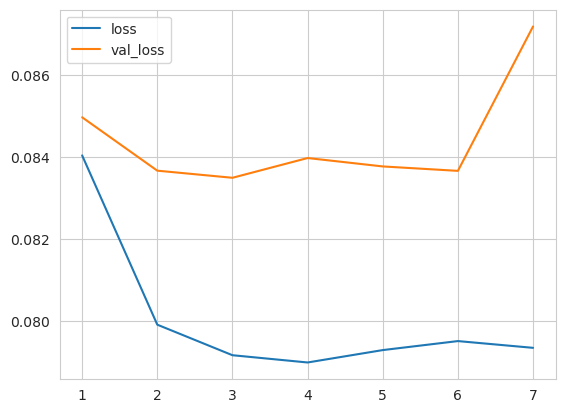
\includegraphics[width=\textwidth]{graphics/model_history_loss_clicks}
    \caption{Only clicks as features}
    \label{fig:model_history_loss_clicks}
  \end{subfigure}
  \hfill
  \begin{subfigure}[b]{0.45\textwidth}
    \centering
    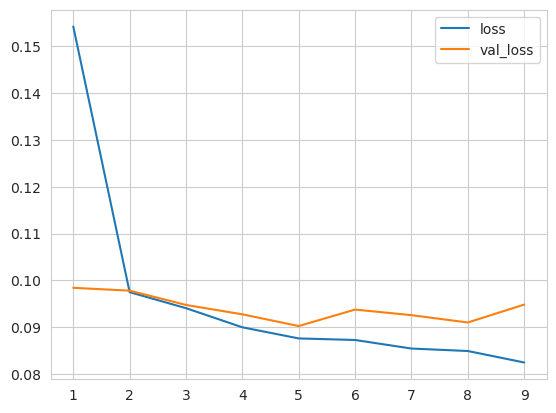
\includegraphics[width=\textwidth]{graphics/model_history_loss_features}
    \caption{Bounding box and click features}
    \label{fig:model_history_loss_features}
  \end{subfigure}
  \hfill
  \begin{subfigure}[b]{0.8\textwidth}
    \centering
    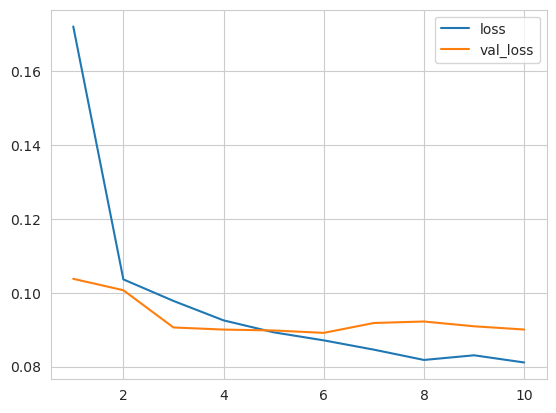
\includegraphics[width=\textwidth]{graphics/model_history_loss_features_shifted}
    \caption{Bounding box and shifted click features}
    \label{fig:model_history_loss_features_shifted}
  \end{subfigure}
  \caption[Training loss vs. validation loss]{Training loss (\ti{loss}, blue) vs. validation loss (\ti{val\_loss}, orange). Horizontal axis is the number of epochs. Vertical axis is the loss as \gls{mse}.}
  \label{fig:model_history_losses}
\end{figure}

\begin{table}[htbp!]
  \small
  \centering
  \begin{tabular}{|l|l|l|l|}
    \hline
    \textbf{Method}      & \textbf{Loss} & \textbf{Validation Loss} & \textbf{Number of epochs} \\
    \hline
    ClickOnly            & 0.0793        & 0.0872                   & 7                         \\
    SelectedFeatures     & 0.0824        & 0.0948                   & 9                         \\
    FeaturesClickShifted & 0.0811        & 0.0900                   & 10                        \\
    \hline
  \end{tabular}
  \caption[Training and validation loss, number of epochs]{Training and validation loss of all three methods, ClickOnly, SelectedFeatures and FeaturesClickShifted}
  \label{tab:model_losses}
\end{table}

\section{Limitations}

Dataset
Dataset is not through different apps, only in one app.
Dataset is not detailed enough in the time steps, or not containing all data
Dataset is not long enough
Dataset has no paid apps or apps with login, which most services require
Dataset has wrong data see \cite{clay}

Preprocessing
Need more time to validate what are the core parameters to predict the next user intent


Model needs more investigation on what data is needed
How many neurons are required to achieve this
Play around with different layers, also Convolutional and pretrained embeddings

